\documentclass[1p]{elsarticle_modified}
%\bibliographystyle{elsarticle-num}

%\usepackage[colorlinks]{hyperref}
%\usepackage{abbrmath_seonhwa} %\Abb, \Ascr, \Acal ,\Abf, \Afrak
\usepackage{amsfonts}
\usepackage{amssymb}
\usepackage{amsmath}
\usepackage{amsthm}
\usepackage{scalefnt}
\usepackage{amsbsy}
\usepackage{kotex}
\usepackage{caption}
\usepackage{subfig}
\usepackage{color}
\usepackage{graphicx}
\usepackage{xcolor} %% white, black, red, green, blue, cyan, magenta, yellow
\usepackage{float}
\usepackage{setspace}
\usepackage{hyperref}

\usepackage{tikz}
\usetikzlibrary{arrows}

\usepackage{multirow}
\usepackage{array} % fixed length table
\usepackage{hhline}

%%%%%%%%%%%%%%%%%%%%%
\makeatletter
\renewcommand*\env@matrix[1][\arraystretch]{%
	\edef\arraystretch{#1}%
	\hskip -\arraycolsep
	\let\@ifnextchar\new@ifnextchar
	\array{*\c@MaxMatrixCols c}}
\makeatother %https://tex.stackexchange.com/questions/14071/how-can-i-increase-the-line-spacing-in-a-matrix
%%%%%%%%%%%%%%%

\usepackage[normalem]{ulem}

\newcommand{\msout}[1]{\ifmmode\text{\sout{\ensuremath{#1}}}\else\sout{#1}\fi}
%SOURCE: \msout is \stkout macro in https://tex.stackexchange.com/questions/20609/strikeout-in-math-mode

\newcommand{\cancel}[1]{
	\ifmmode
	{\color{red}\msout{#1}}
	\else
	{\color{red}\sout{#1}}
	\fi
}

\newcommand{\add}[1]{
	{\color{blue}\uwave{#1}}
}

\newcommand{\replace}[2]{
	\ifmmode
	{\color{red}\msout{#1}}{\color{blue}\uwave{#2}}
	\else
	{\color{red}\sout{#1}}{\color{blue}\uwave{#2}}
	\fi
}

\newcommand{\Sol}{\mathcal{S}} %segment
\newcommand{\D}{D} %diagram
\newcommand{\A}{\mathcal{A}} %arc


%%%%%%%%%%%%%%%%%%%%%%%%%%%%%5 test

\def\sl{\operatorname{\textup{SL}}(2,\Cbb)}
\def\psl{\operatorname{\textup{PSL}}(2,\Cbb)}
\def\quan{\mkern 1mu \triangleright \mkern 1mu}

\theoremstyle{definition}
\newtheorem{thm}{Theorem}[section]
\newtheorem{prop}[thm]{Proposition}
\newtheorem{lem}[thm]{Lemma}
\newtheorem{ques}[thm]{Question}
\newtheorem{cor}[thm]{Corollary}
\newtheorem{defn}[thm]{Definition}
\newtheorem{exam}[thm]{Example}
\newtheorem{rmk}[thm]{Remark}
\newtheorem{alg}[thm]{Algorithm}

\newcommand{\I}{\sqrt{-1}}
\begin{document}

%\begin{frontmatter}
%
%\title{Boundary parabolic representations of knots up to 8 crossings}
%
%%% Group authors per affiliation:
%\author{Yunhi Cho} 
%\address{Department of Mathematics, University of Seoul, Seoul, Korea}
%\ead{yhcho@uos.ac.kr}
%
%
%\author{Seonhwa Kim} %\fnref{s_kim}}
%\address{Center for Geometry and Physics, Institute for Basic Science, Pohang, 37673, Korea}
%\ead{ryeona17@ibs.re.kr}
%
%\author{Hyuk Kim}
%\address{Department of Mathematical Sciences, Seoul National University, Seoul 08826, Korea}
%\ead{hyukkim@snu.ac.kr}
%
%\author{Seokbeom Yoon}
%\address{Department of Mathematical Sciences, Seoul National University, Seoul, 08826,  Korea}
%\ead{sbyoon15@snu.ac.kr}
%
%\begin{abstract}
%We find all boundary parabolic representation of knots up to 8 crossings.
%
%\end{abstract}
%\begin{keyword}
%    \MSC[2010] 57M25 
%\end{keyword}
%
%\end{frontmatter}

%\linenumbers
%\tableofcontents
%
\newcommand\colored[1]{\textcolor{white}{\rule[-0.35ex]{0.8em}{1.4ex}}\kern-0.8em\color{red} #1}%
%\newcommand\colored[1]{\textcolor{white}{ #1}\kern-2.17ex	\textcolor{white}{ #1}\kern-1.81ex	\textcolor{white}{ #1}\kern-2.15ex\color{red}#1	}

{\Large $\underline{10_{43}~(K10a_{52})}$}

\setlength{\tabcolsep}{10pt}
\renewcommand{\arraystretch}{1.6}
\vspace{1cm}\begin{tabular}{m{100pt}>{\centering\arraybackslash}m{274pt}}
\multirow{5}{120pt}{
	\centering
	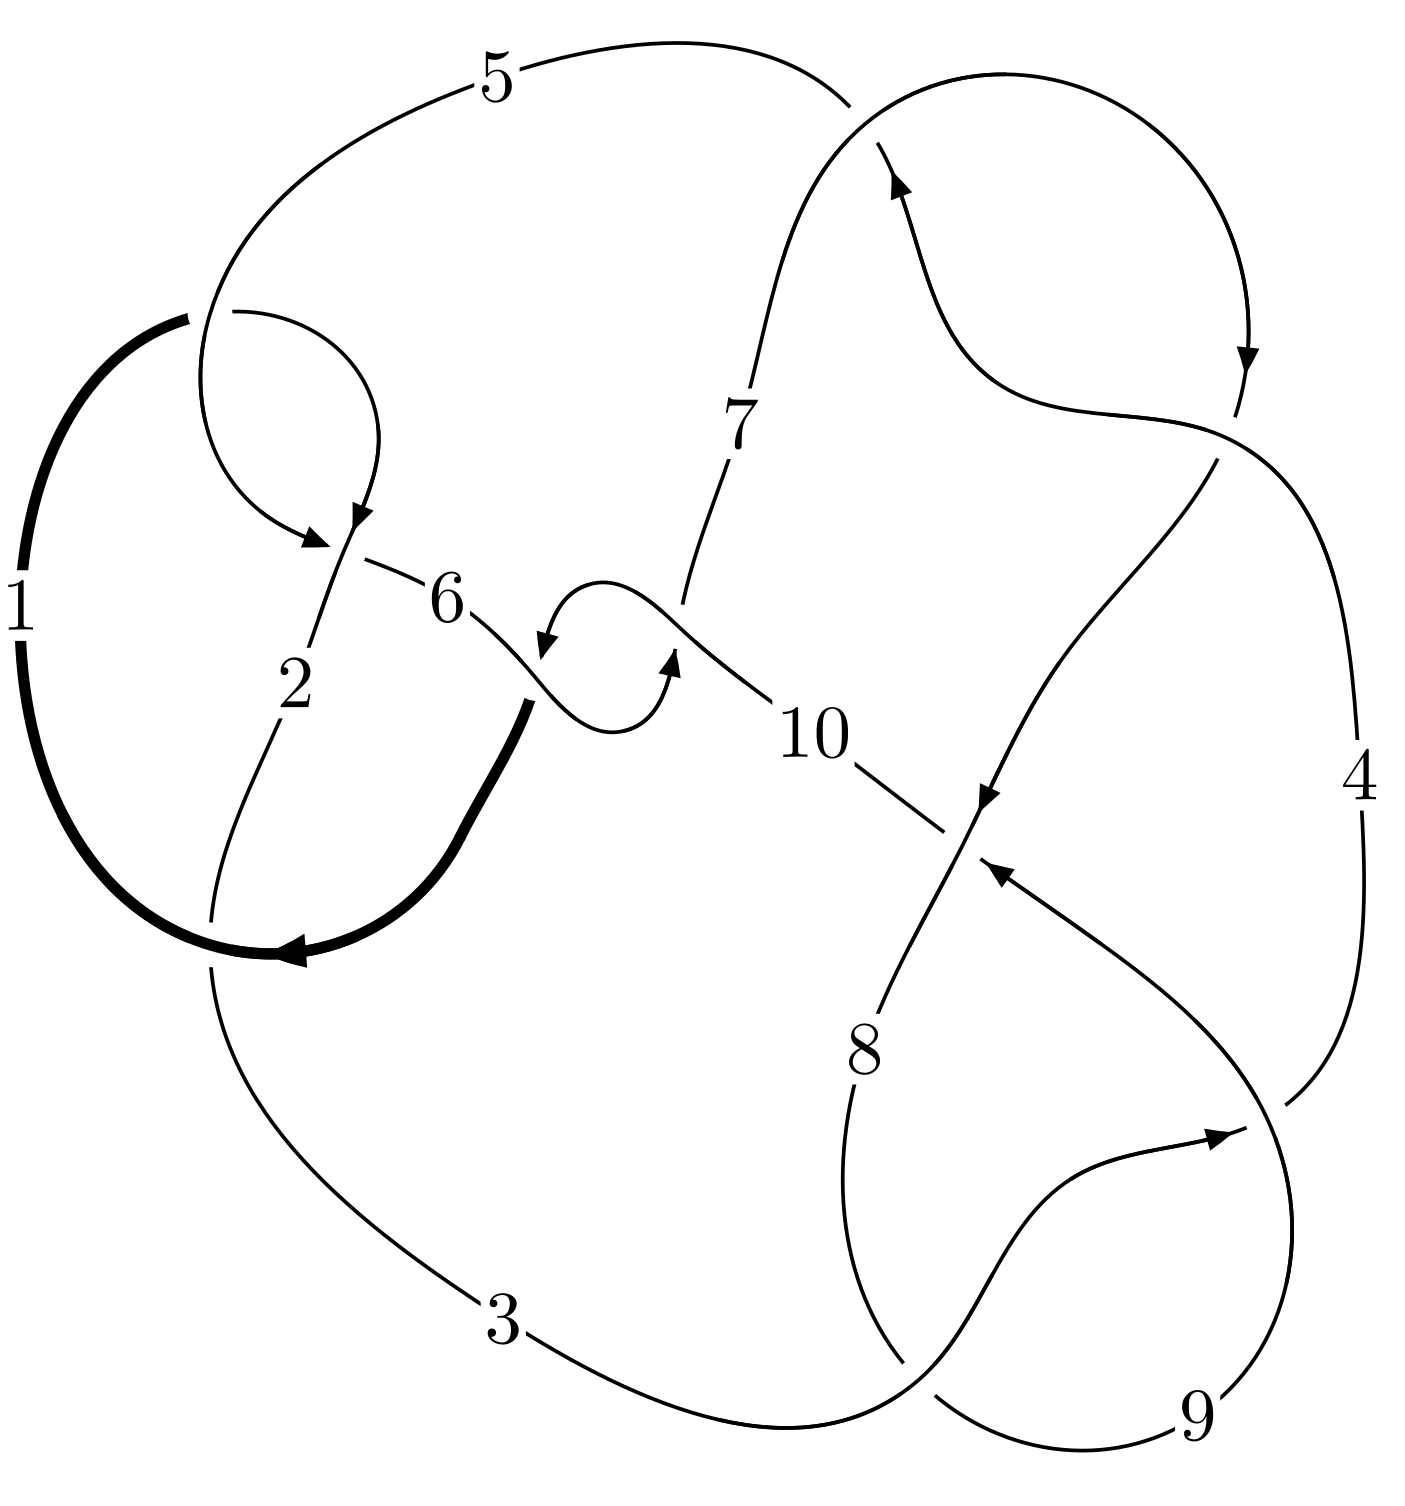
\includegraphics[width=112pt]{../../../GIT/diagram.site/Diagrams/png/127_10_43.png}\\
\ \ \ A knot diagram\footnotemark}&
\allowdisplaybreaks
\textbf{Linearized knot diagam} \\
\cline{2-2}
 &
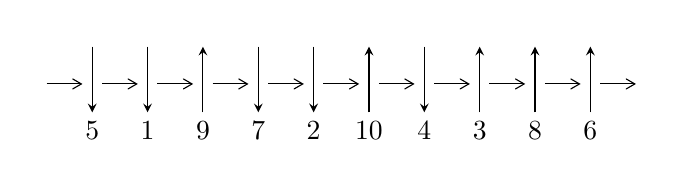
\begin{tikzpicture}[x=20pt, y=17pt]
	% nodes
	\node (C0) at (0, 0) {};
	\node (C1) at (1, 0) {};
	\node (C1U) at (1, +1) {};
	\node (C1D) at (1, -1) {5};

	\node (C2) at (2, 0) {};
	\node (C2U) at (2, +1) {};
	\node (C2D) at (2, -1) {1};

	\node (C3) at (3, 0) {};
	\node (C3U) at (3, +1) {};
	\node (C3D) at (3, -1) {9};

	\node (C4) at (4, 0) {};
	\node (C4U) at (4, +1) {};
	\node (C4D) at (4, -1) {7};

	\node (C5) at (5, 0) {};
	\node (C5U) at (5, +1) {};
	\node (C5D) at (5, -1) {2};

	\node (C6) at (6, 0) {};
	\node (C6U) at (6, +1) {};
	\node (C6D) at (6, -1) {10};

	\node (C7) at (7, 0) {};
	\node (C7U) at (7, +1) {};
	\node (C7D) at (7, -1) {4};

	\node (C8) at (8, 0) {};
	\node (C8U) at (8, +1) {};
	\node (C8D) at (8, -1) {3};

	\node (C9) at (9, 0) {};
	\node (C9U) at (9, +1) {};
	\node (C9D) at (9, -1) {8};

	\node (C10) at (10, 0) {};
	\node (C10U) at (10, +1) {};
	\node (C10D) at (10, -1) {6};
	\node (C11) at (11, 0) {};

	% arrows
	\draw[->,>={angle 60}]
	(C0) edge (C1) (C1) edge (C2) (C2) edge (C3) (C3) edge (C4) (C4) edge (C5) (C5) edge (C6) (C6) edge (C7) (C7) edge (C8) (C8) edge (C9) (C9) edge (C10) (C10) edge (C11) ;	\draw[->,>=stealth]
	(C1U) edge (C1D) (C2U) edge (C2D) (C3D) edge (C3U) (C4U) edge (C4D) (C5U) edge (C5D) (C6D) edge (C6U) (C7U) edge (C7D) (C8D) edge (C8U) (C9D) edge (C9U) (C10D) edge (C10U) ;
	\end{tikzpicture} \\
\hhline{~~} \\& 
\textbf{Solving Sequence} \\ \cline{2-2} 
 &
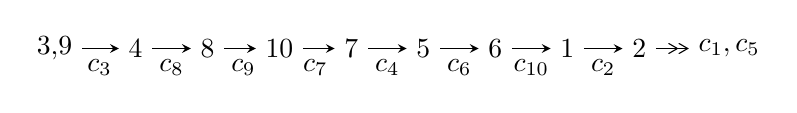
\begin{tikzpicture}[x=26pt, y=7pt]
	% node
	\node (A0) at (-1/8, 0) {3,9};
	\node (A1) at (1, 0) {4};
	\node (A2) at (2, 0) {8};
	\node (A3) at (3, 0) {10};
	\node (A4) at (4, 0) {7};
	\node (A5) at (5, 0) {5};
	\node (A6) at (6, 0) {6};
	\node (A7) at (7, 0) {1};
	\node (A8) at (8, 0) {2};
	\node (C1) at (1/2, -1) {$c_{3}$};
	\node (C2) at (3/2, -1) {$c_{8}$};
	\node (C3) at (5/2, -1) {$c_{9}$};
	\node (C4) at (7/2, -1) {$c_{7}$};
	\node (C5) at (9/2, -1) {$c_{4}$};
	\node (C6) at (11/2, -1) {$c_{6}$};
	\node (C7) at (13/2, -1) {$c_{10}$};
	\node (C8) at (15/2, -1) {$c_{2}$};
	\node (A9) at (37/4, 0) {$c_{1},c_{5}$};

	% edge
	\draw[->,>=stealth]	
	(A0) edge (A1) (A1) edge (A2) (A2) edge (A3) (A3) edge (A4) (A4) edge (A5) (A5) edge (A6) (A6) edge (A7) (A7) edge (A8) ;
	\draw[->>,>={angle 60}]	
	(A8) edge (A9);
\end{tikzpicture} \\ 

\end{tabular} \\

\footnotetext{
The image of knot diagram is generated by the software ``\textbf{Draw programme}" developed by Andrew Bartholomew(\url{http://www.layer8.co.uk/maths/draw/index.htm\#Running-draw}), where we modified some parts for our purpose(\url{https://github.com/CATsTAILs/LinksPainter}).
}\phantom \\ \newline 
\centering \textbf{Ideals for irreducible components\footnotemark of $X_{\text{par}}$} 
 
\begin{align*}
I^u_{1}&=\langle 
u^{36}- u^{35}+\cdots- u^2+1\rangle \\
\\
\end{align*}
\raggedright * 1 irreducible components of $\dim_{\mathbb{C}}=0$, with total 36 representations.\\
\footnotetext{All coefficients of polynomials are rational numbers. But the coefficients are sometimes approximated in decimal forms when there is not enough margin.}
\newpage
\renewcommand{\arraystretch}{1}
\centering \section*{I. $I^u_{1}= \langle u^{36}- u^{35}+\cdots- u^2+1 \rangle$}
\flushleft \textbf{(i) Arc colorings}\\
\begin{tabular}{m{7pt} m{180pt} m{7pt} m{180pt} }
\flushright $a_{3}=$&$\begin{pmatrix}1\\0\end{pmatrix}$ \\
\flushright $a_{9}=$&$\begin{pmatrix}0\\u\end{pmatrix}$ \\
\flushright $a_{4}=$&$\begin{pmatrix}1\\- u^2\end{pmatrix}$ \\
\flushright $a_{8}=$&$\begin{pmatrix}- u\\u\end{pmatrix}$ \\
\flushright $a_{10}=$&$\begin{pmatrix}u^3\\- u^3+u\end{pmatrix}$ \\
\flushright $a_{7}=$&$\begin{pmatrix}- u^3\\u^5- u^3+u\end{pmatrix}$ \\
\flushright $a_{5}=$&$\begin{pmatrix}u^6- u^4+1\\- u^8+2 u^6-2 u^4\end{pmatrix}$ \\
\flushright $a_{6}=$&$\begin{pmatrix}- u^{11}+2 u^9-2 u^7- u^3\\u^{11}-3 u^9+4 u^7- u^5- u^3+u\end{pmatrix}$ \\
\flushright $a_{1}=$&$\begin{pmatrix}u^{19}-4 u^{17}+8 u^{15}-8 u^{13}+5 u^{11}-2 u^9+2 u^7+u^3\\- u^{19}+5 u^{17}-12 u^{15}+15 u^{13}-9 u^{11}- u^9+4 u^7-2 u^5- u^3+u\end{pmatrix}$ \\
\flushright $a_{2}=$&$\begin{pmatrix}- u^{33}+8 u^{31}+\cdots+2 u^3- u\\u^{35}-9 u^{33}+\cdots- u^3+u\end{pmatrix}$\\&\end{tabular}
\flushleft \textbf{(ii) Obstruction class $= -1$}\\~\\
\flushleft \textbf{(iii) Cusp Shapes $= -4 u^{35}+40 u^{33}-4 u^{32}-192 u^{31}+36 u^{30}+564 u^{29}-156 u^{28}-1092 u^{27}+412 u^{26}+1380 u^{25}-712 u^{24}-980 u^{23}+792 u^{22}+16 u^{21}-480 u^{20}+732 u^{19}-16 u^{18}-680 u^{17}+280 u^{16}+112 u^{15}-188 u^{14}+272 u^{13}-12 u^{12}-216 u^{11}+80 u^{10}-36 u^8+80 u^7-8 u^6-32 u^5+8 u^4-4 u^3+8 u+2$}\\~\\
\newpage\renewcommand{\arraystretch}{1}
\flushleft \textbf{(iv) u-Polynomials at the component}\newline \\
\begin{tabular}{m{50pt}|m{274pt}}
Crossings & \hspace{64pt}u-Polynomials at each crossing \\
\hline $$\begin{aligned}c_{1},c_{5}\end{aligned}$$&$\begin{aligned}
&u^{36}+u^{35}+\cdots- u^2+1
\end{aligned}$\\
\hline $$\begin{aligned}c_{2}\end{aligned}$$&$\begin{aligned}
&u^{36}+19 u^{35}+\cdots+2 u+1
\end{aligned}$\\
\hline $$\begin{aligned}c_{3},c_{8}\end{aligned}$$&$\begin{aligned}
&u^{36}- u^{35}+\cdots- u^2+1
\end{aligned}$\\
\hline $$\begin{aligned}c_{4},c_{7}\end{aligned}$$&$\begin{aligned}
&u^{36}-3 u^{35}+\cdots-22 u+5
\end{aligned}$\\
\hline $$\begin{aligned}c_{6},c_{10}\end{aligned}$$&$\begin{aligned}
&u^{36}+3 u^{35}+\cdots+22 u+5
\end{aligned}$\\
\hline $$\begin{aligned}c_{9}\end{aligned}$$&$\begin{aligned}
&u^{36}-19 u^{35}+\cdots-2 u+1
\end{aligned}$\\
\hline
\end{tabular}\\~\\
\newpage\renewcommand{\arraystretch}{1}
\flushleft \textbf{(v) Riley Polynomials at the component}\newline \\
\begin{tabular}{m{50pt}|m{274pt}}
Crossings & \hspace{64pt}Riley Polynomials at each crossing \\
\hline $$\begin{aligned}c_{1},c_{3},c_{5}\\c_{8}\end{aligned}$$&$\begin{aligned}
&y^{36}-19 y^{35}+\cdots-2 y+1
\end{aligned}$\\
\hline $$\begin{aligned}c_{2},c_{9}\end{aligned}$$&$\begin{aligned}
&y^{36}-3 y^{35}+\cdots+2 y+1
\end{aligned}$\\
\hline $$\begin{aligned}c_{4},c_{6},c_{7}\\c_{10}\end{aligned}$$&$\begin{aligned}
&y^{36}+25 y^{35}+\cdots-154 y+25
\end{aligned}$\\
\hline
\end{tabular}\\~\\
\newpage\flushleft \textbf{(vi) Complex Volumes and Cusp Shapes}
$$\begin{array}{c|c|c}  
\text{Solutions to }I^u_{1}& \I (\text{vol} + \sqrt{-1}CS) & \text{Cusp shape}\\
 \hline 
\begin{aligned}
u &= \phantom{-}0.805609 + 0.585926 I\end{aligned}
 & -5.78512 + 6.60899 I & -5.22618 - 6.99003 I \\ \hline\begin{aligned}
u &= \phantom{-}0.805609 - 0.585926 I\end{aligned}
 & -5.78512 - 6.60899 I & -5.22618 + 6.99003 I \\ \hline\begin{aligned}
u &= -0.973666 + 0.342560 I\end{aligned}
 & \phantom{-0.000000 } -3.75301 I & \phantom{-0.000000 -}0. + 6.73664 I \\ \hline\begin{aligned}
u &= -0.973666 - 0.342560 I\end{aligned}
 & \phantom{-0.000000 -}3.75301 I & \phantom{-0.000000 } 0. - 6.73664 I \\ \hline\begin{aligned}
u &= -0.771553 + 0.550437 I\end{aligned}
 & -2.48653 - 2.21040 I & -2.18679 + 3.72055 I \\ \hline\begin{aligned}
u &= -0.771553 - 0.550437 I\end{aligned}
 & -2.48653 + 2.21040 I & -2.18679 - 3.72055 I \\ \hline\begin{aligned}
u &= \phantom{-}0.733643 + 0.592284 I\end{aligned}
 & -5.99129 - 1.96554 I & -6.00564 + 0.22737 I \\ \hline\begin{aligned}
u &= \phantom{-}0.733643 - 0.592284 I\end{aligned}
 & -5.99129 + 1.96554 I & -6.00564 - 0.22737 I \\ \hline\begin{aligned}
u &= \phantom{-}0.879174 + 0.103222 I\end{aligned}
 & \phantom{-}1.48890 + 0.27307 I & \phantom{-}6.50261 - 0.38004 I \\ \hline\begin{aligned}
u &= \phantom{-}0.879174 - 0.103222 I\end{aligned}
 & \phantom{-}1.48890 - 0.27307 I & \phantom{-}6.50261 + 0.38004 I \\ \hline\begin{aligned}
u &= -1.079360 + 0.331184 I\end{aligned}
 & \phantom{-0.000000 } -3.70794 I & \phantom{-0.000000 -}0. + 4.78665 I \\ \hline\begin{aligned}
u &= -1.079360 - 0.331184 I\end{aligned}
 & \phantom{-0.000000 -}3.70794 I & \phantom{-0.000000 } 0. - 4.78665 I \\ \hline\begin{aligned}
u &= \phantom{-}0.193860 + 0.787757 I\end{aligned}
 & -2.88545 - 7.72472 I & -3.24945 + 5.61903 I \\ \hline\begin{aligned}
u &= \phantom{-}0.193860 - 0.787757 I\end{aligned}
 & -2.88545 + 7.72472 I & -3.24945 - 5.61903 I \\ \hline\begin{aligned}
u &= \phantom{-}1.169940 + 0.367759 I\end{aligned}
 & \phantom{-}3.90881 + 0.64400 I & \phantom{-}5.19682 - 0.84878 I \\ \hline\begin{aligned}
u &= \phantom{-}1.169940 - 0.367759 I\end{aligned}
 & \phantom{-}3.90881 - 0.64400 I & \phantom{-}5.19682 + 0.84878 I \\ \hline\begin{aligned}
u &= -0.176866 + 0.751609 I\end{aligned}
 & \phantom{-0.000000 -}2.99647 I & \phantom{-0.000000 } 0. - 2.49060 I \\ \hline\begin{aligned}
u &= -0.176866 - 0.751609 I\end{aligned}
 & \phantom{-0.000000 } -2.99647 I & \phantom{-0.000000 -}0. + 2.49060 I \\ \hline\begin{aligned}
u &= \phantom{-}0.241156 + 0.725408 I\end{aligned}
 & -3.90881 + 0.64400 I & -5.19682 - 0.84878 I \\ \hline\begin{aligned}
u &= \phantom{-}0.241156 - 0.725408 I\end{aligned}
 & -3.90881 - 0.64400 I & -5.19682 + 0.84878 I \\ \hline\begin{aligned}
u &= -1.188280 + 0.342283 I\end{aligned}
 & \phantom{-}1.27958 + 4.07135 I & \phantom{-}1.88452 - 2.88119 I \\ \hline\begin{aligned}
u &= -1.188280 - 0.342283 I\end{aligned}
 & \phantom{-}1.27958 - 4.07135 I & \phantom{-}1.88452 + 2.88119 I \\ \hline\begin{aligned}
u &= -0.038116 + 0.743633 I\end{aligned}
 & \phantom{-}2.48653 + 2.21040 I & \phantom{-}2.18679 - 3.72055 I \\ \hline\begin{aligned}
u &= -0.038116 - 0.743633 I\end{aligned}
 & \phantom{-}2.48653 - 2.21040 I & \phantom{-}2.18679 + 3.72055 I \\ \hline\begin{aligned}
u &= \phantom{-}1.143830 + 0.521070 I\end{aligned}
 & -1.27958 + 4.07135 I & -1.88452 - 2.88119 I \\ \hline\begin{aligned}
u &= \phantom{-}1.143830 - 0.521070 I\end{aligned}
 & -1.27958 - 4.07135 I & -1.88452 + 2.88119 I \\ \hline\begin{aligned}
u &= \phantom{-}1.184710 + 0.434081 I\end{aligned}
 & \phantom{-}5.99129 + 1.96554 I & \phantom{-}6.00564 - 0.22737 I \\ \hline\begin{aligned}
u &= \phantom{-}1.184710 - 0.434081 I\end{aligned}
 & \phantom{-}5.99129 - 1.96554 I & \phantom{-}6.00564 + 0.22737 I \\ \hline\begin{aligned}
u &= -1.184420 + 0.463218 I\end{aligned}
 & \phantom{-}5.78512 - 6.60899 I & \phantom{-}5.22618 + 6.99003 I \\ \hline\begin{aligned}
u &= -1.184420 - 0.463218 I\end{aligned}
 & \phantom{-}5.78512 + 6.60899 I & \phantom{-}5.22618 - 6.99003 I\\
 \hline 
 \end{array}$$\newpage$$\begin{array}{c|c|c}  
\text{Solutions to }I^u_{1}& \I (\text{vol} + \sqrt{-1}CS) & \text{Cusp shape}\\
 \hline 
\begin{aligned}
u &= -1.168380 + 0.513346 I\end{aligned}
 & \phantom{-}2.88545 - 7.72472 I & \phantom{-}3.24945 + 5.61903 I \\ \hline\begin{aligned}
u &= -1.168380 - 0.513346 I\end{aligned}
 & \phantom{-}2.88545 + 7.72472 I & \phantom{-}3.24945 - 5.61903 I \\ \hline\begin{aligned}
u &= \phantom{-}1.175040 + 0.526945 I\end{aligned}
 & \phantom{-0.000000 -}12.6026 I & \phantom{-0.000000 } 0. - 8.81146 I \\ \hline\begin{aligned}
u &= \phantom{-}1.175040 - 0.526945 I\end{aligned}
 & \phantom{-0.000000 } -12.6026 I & \phantom{-0.000000 -}0. + 8.81146 I \\ \hline\begin{aligned}
u &= -0.446315 + 0.412227 I\end{aligned}
 & -1.48890 + 0.27307 I & -6.50261 - 0.38004 I \\ \hline\begin{aligned}
u &= -0.446315 - 0.412227 I\end{aligned}
 & -1.48890 - 0.27307 I & -6.50261 + 0.38004 I\\
 \hline 
 \end{array}$$\newpage
\newpage\renewcommand{\arraystretch}{1}
\centering \section*{ II. u-Polynomials}
\begin{tabular}{m{50pt}|m{274pt}}
Crossings & \hspace{64pt}u-Polynomials at each crossing \\
\hline $$\begin{aligned}c_{1},c_{5}\end{aligned}$$&$\begin{aligned}
&u^{36}+u^{35}+\cdots- u^2+1
\end{aligned}$\\
\hline $$\begin{aligned}c_{2}\end{aligned}$$&$\begin{aligned}
&u^{36}+19 u^{35}+\cdots+2 u+1
\end{aligned}$\\
\hline $$\begin{aligned}c_{3},c_{8}\end{aligned}$$&$\begin{aligned}
&u^{36}- u^{35}+\cdots- u^2+1
\end{aligned}$\\
\hline $$\begin{aligned}c_{4},c_{7}\end{aligned}$$&$\begin{aligned}
&u^{36}-3 u^{35}+\cdots-22 u+5
\end{aligned}$\\
\hline $$\begin{aligned}c_{6},c_{10}\end{aligned}$$&$\begin{aligned}
&u^{36}+3 u^{35}+\cdots+22 u+5
\end{aligned}$\\
\hline $$\begin{aligned}c_{9}\end{aligned}$$&$\begin{aligned}
&u^{36}-19 u^{35}+\cdots-2 u+1
\end{aligned}$\\
\hline
\end{tabular}\newpage\renewcommand{\arraystretch}{1}
\centering \section*{ III. Riley Polynomials}
\begin{tabular}{m{50pt}|m{274pt}}
Crossings & \hspace{64pt}Riley Polynomials at each crossing \\
\hline $$\begin{aligned}c_{1},c_{3},c_{5}\\c_{8}\end{aligned}$$&$\begin{aligned}
&y^{36}-19 y^{35}+\cdots-2 y+1
\end{aligned}$\\
\hline $$\begin{aligned}c_{2},c_{9}\end{aligned}$$&$\begin{aligned}
&y^{36}-3 y^{35}+\cdots+2 y+1
\end{aligned}$\\
\hline $$\begin{aligned}c_{4},c_{6},c_{7}\\c_{10}\end{aligned}$$&$\begin{aligned}
&y^{36}+25 y^{35}+\cdots-154 y+25
\end{aligned}$\\
\hline
\end{tabular}
\vskip 2pc
\end{document}